\documentclass[aspectratio=169,10pt]{beamer}

\usetheme{Madrid}
\usecolortheme{seahorse}

\usepackage{amsmath}
\usepackage{amssymb}
\usepackage{amsthm}
\usepackage{graphicx}
\usepackage{listings}
\usepackage{xcolor}
\usepackage{hyperref}
\usepackage{float}

\graphicspath{{figures/}}

% Configure listings style for Python code
\lstset{
  basicstyle=\ttfamily\scriptsize,
  breaklines=true,
  commentstyle=\color{green!50!black}\itshape,
  keywordstyle=\color{blue}\bfseries,
  stringstyle=\color{red},
  showstringspaces=false,
  numbers=left,
  numberstyle=\tiny\color{gray},
  frame=single,
  framerule=1pt,
  rulecolor=\color{gray},
  xleftmargin=8pt,
  xrightmargin=8pt,
  aboveskip=8pt,
  belowskip=8pt
}

\setbeamertemplate{footline}[frame number]
\setbeamertemplate{caption}[numbered]

% Title page
\title{Approximation of Fixed Point Mappings}
\subtitle{Pathak (2018) -- Chapter 6e\\
Applications of Fixed Point Theorems}
\author{Lecture Notes}
\date{\today}

\begin{document}

% Title Frame
\frame{\titlepage}

% Table of Contents
\begin{frame}{Contents}
  \tableofcontents
\end{frame}

%===============================================================================
\section{Introduction to Fixed Point Approximation}
%===============================================================================

\begin{frame}[allowframebreaks]{Fixed Point Mappings and Iteration}
  \begin{definition}[Fixed Point]
    Let $(X, \|\cdot\|)$ be a Banach space and $T: D \subseteq X \to X$ be a mapping.
    A point $x^* \in D$ is called a \textbf{fixed point} of $T$ if
    \[
      T(x^*) = x^*.
    \]
  \end{definition}

  \vspace{0.3cm}

  \begin{definition}[Fixed Point Approximation]
    Given a mapping $T$ with a fixed point $x^*$, an \textbf{approximation sequence}
    $\{x_n\}$ is defined recursively by
    \[
      x_{n+1} = T(x_n), \quad n = 0, 1, 2, \ldots
    \]
    where $x_0 \in D$ is an initial guess.
  \end{definition}

  \vspace{0.3cm}

  \begin{theorem}[Existence and Uniqueness]
    If $T: D \to D$ is a continuous mapping on a compact set $D$ in a Banach space,
    then $T$ has at least one fixed point.
  \end{theorem}

  \framebreak

  \begin{center}
    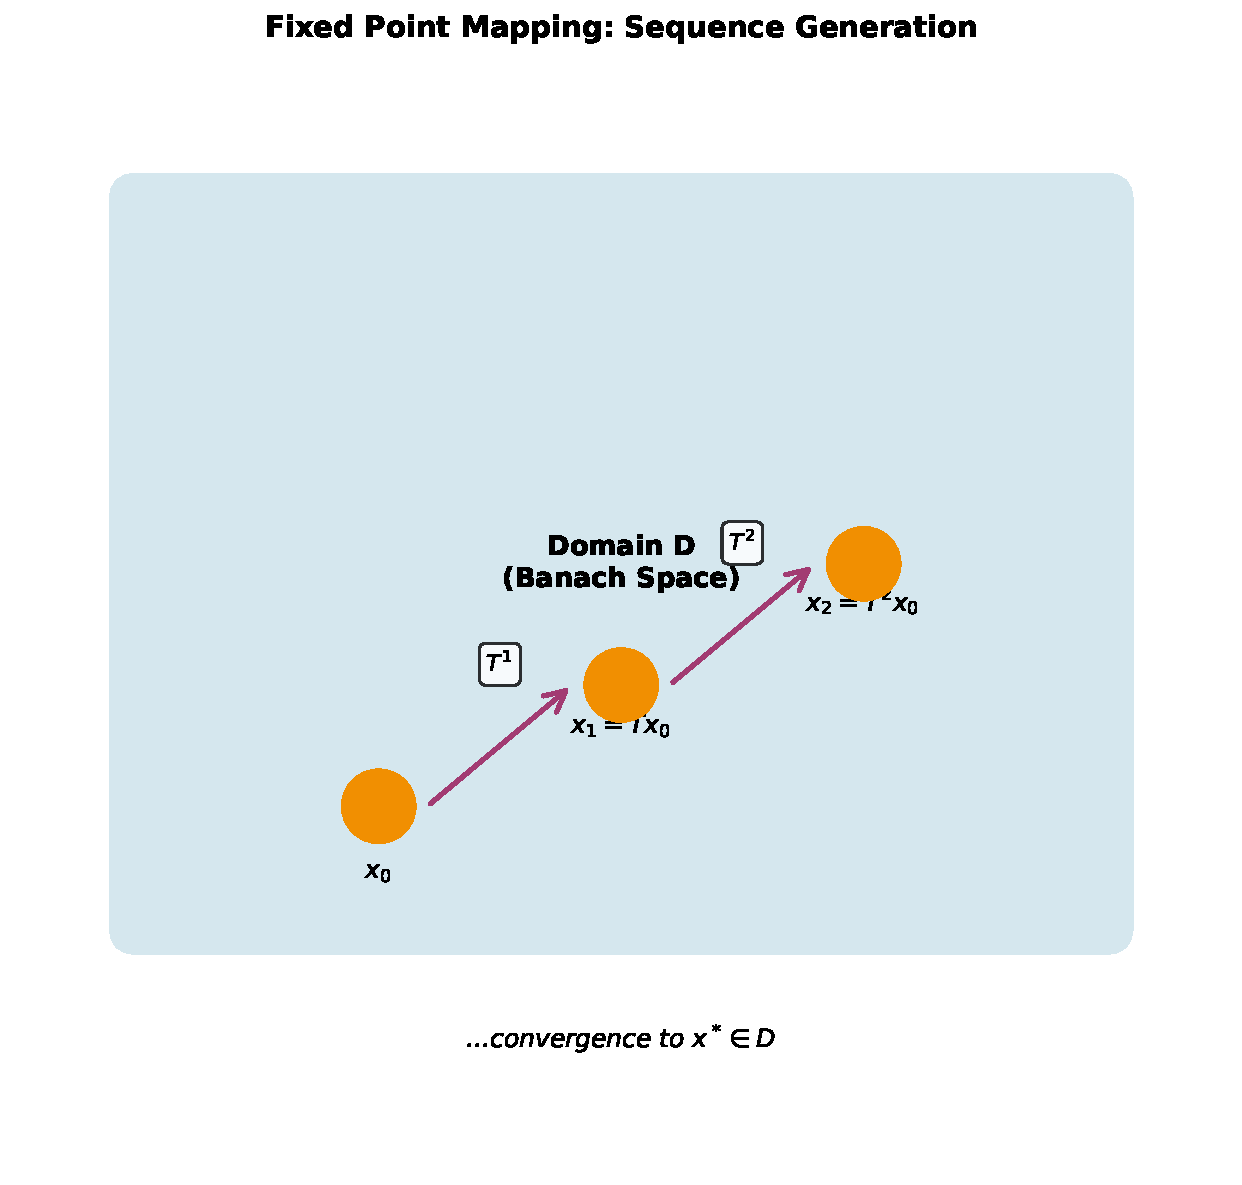
\includegraphics[width=0.9\textwidth]{fig_05_domain_diagram.pdf}
  \end{center}
\end{frame}

\begin{frame}{Basic Iterative Scheme}
  \begin{block}{Picard Iteration}
    The most basic approach to approximate a fixed point is the Picard iteration:
    \[
      x_{n+1} = T(x_n), \quad n = 0, 1, 2, \ldots
    \]
  \end{block}

  \vspace{0.4cm}

  \textbf{Key Questions:}
  \begin{enumerate}
    \item Does the sequence $\{x_n\}$ converge?
    \item If it converges, does it converge to a fixed point?
    \item What is the rate of convergence?
    \item How many iterations are needed for a desired accuracy?
  \end{enumerate}

  \vspace{0.4cm}

  \begin{remark}
    The convergence depends on properties of $T$ (continuity, contractiveness, etc.)
    and the structure of the domain $D$.
  \end{remark}
\end{frame}

%===============================================================================
\section{Contraction Mapping Theorem}
%===============================================================================

\begin{frame}{Contraction Mappings}
  \begin{definition}[Contraction Mapping]
    A mapping $T: D \subseteq X \to X$ is a \textbf{contraction mapping} (or $\lambda$-contraction)
    if there exists a constant $0 \leq \lambda < 1$ such that
    \[
      \|T(x) - T(y)\| \leq \lambda \|x - y\|
      \quad \text{for all } x, y \in D.
    \]
    The constant $\lambda$ is called the \textbf{contraction rate}.
  \end{definition}

  \vspace{0.4cm}

  \begin{block}{Properties}
    \item Every contraction is continuous.
    \item A contraction is uniformly continuous.
    \item The contraction rate measures how fast distances shrink.
  \end{block}
\end{frame}

\begin{frame}{Banach Contraction Mapping Theorem}
  \begin{theorem}[Banach (1922)]
    Let $(X, \|\cdot\|)$ be a complete metric space and $T: X \to X$ be a contraction
    mapping with contraction rate $0 \leq \lambda < 1$. Then:
    \begin{enumerate}
      \item $T$ has a unique fixed point $x^* \in X$.
      \item For any initial point $x_0 \in X$, the sequence $\{x_n\}$ defined by
            $x_{n+1} = T(x_n)$ converges to $x^*$.
      \item The error estimate is:
            \[
              \|x_n - x^*\| \leq \lambda^n \|x_0 - x^*\|.
            \]
    \end{enumerate}
  \end{theorem}

  \vspace{0.3cm}

  \begin{corollary}[A Priori Error Bound]
    Before computing $x_n$, we can estimate:
    \[
      \|x_n - x^*\| \leq \frac{\lambda^n}{1 - \lambda} \|x_1 - x_0\|.
    \]
  \end{corollary}
\end{frame}

\begin{frame}{Visual Illustration of Contraction Mappings}
  \begin{center}
    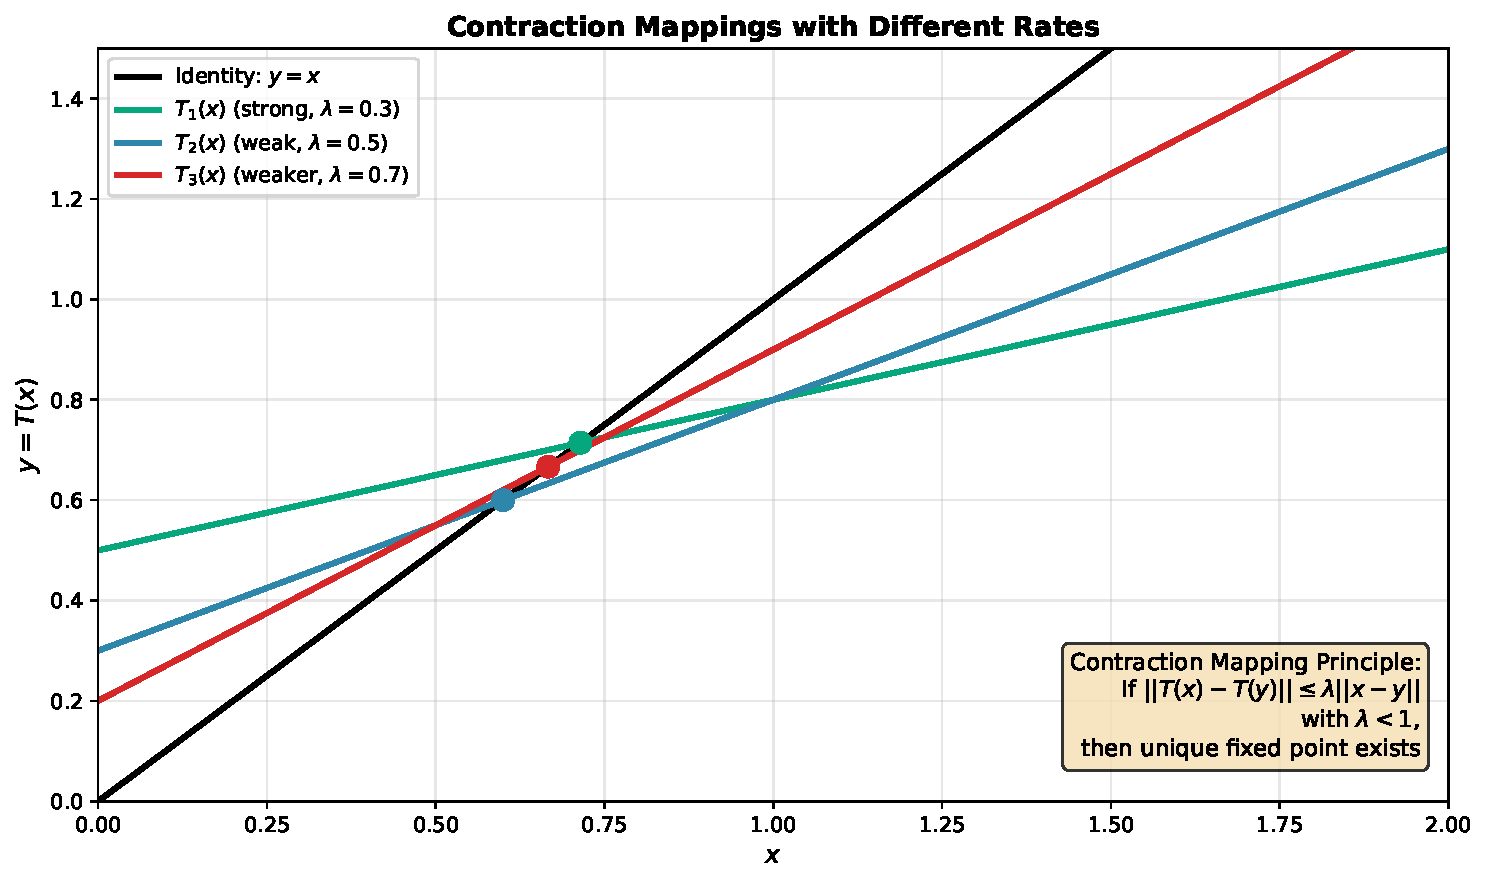
\includegraphics[width=0.95\textwidth]{fig_06_contraction_mapping.pdf}
  \end{center}

  \vspace{0.2cm}
  \small
  The graphical interpretation shows the cobweb diagram where iterates
  converge to the intersection of $y=x$ and $y=T(x)$ (the fixed point).
\end{frame}

%===============================================================================
\section{Convergence Analysis}
%===============================================================================

\begin{frame}[allowframebreaks]{Linear and Nonlinear Convergence}
  \begin{definition}[Order of Convergence]
    A sequence $\{x_n\}$ converges to $x^*$ with \textbf{order} $p$ if:
    \[
      \|x_{n+1} - x^*\| \leq C \|x_n - x^*\|^p
    \]
    for some constant $C > 0$ and all $n$ sufficiently large.
  \end{definition}

  \vspace{0.3cm}

  \begin{itemize}
    \item \textbf{Linear convergence:} $p = 1$ with $0 < C < 1$
    \item \textbf{Superlinear convergence:} $p = 1$ with $C = 0$
    \item \textbf{Quadratic convergence:} $p = 2$
    \item \textbf{Superquadratic convergence:} $p > 2$
  \end{itemize}

  \framebreak

  \begin{center}
    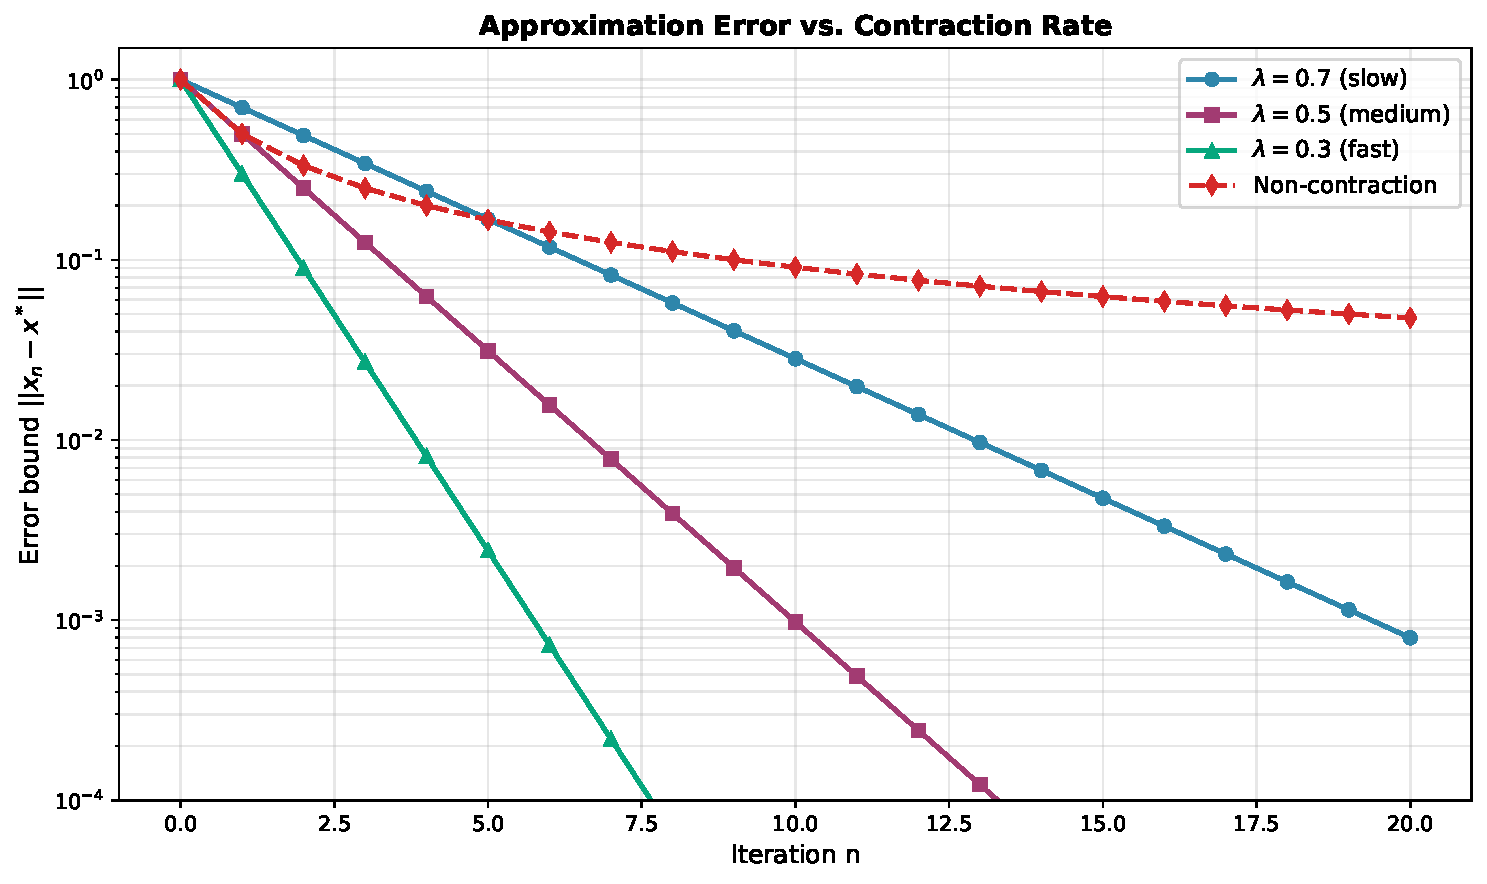
\includegraphics[width=0.95\textwidth]{fig_03_approximation_error.pdf}
  \end{center}

  \vspace{0.2cm}
  \small
  Faster contraction rates lead to exponentially faster error reduction.
\end{frame}

\begin{frame}{Error Bounds and Stopping Criteria}
  \begin{block}{Residual Error}
    At iteration $m$, define the residual error:
    \[
      R_m = \|x_{m+1} - T(x_m)\| = \|x_{m+1} - x_{m+1}\| = 0 \quad \text{(by construction)}
    \]

    More generally, we measure:
    \[
      R_m = \|F(x_m)\|
    \]
    where $F(x) = x - T(x)$ is the \textbf{residual operator}.
  \end{block}

  \vspace{0.4cm}

  \begin{block}{Stopping Criteria}
    Common criteria to terminate iteration:
    \begin{enumerate}
      \item $\|x_{n+1} - x_n\| < \epsilon$ (successive approximation)
      \item $\|F(x_n)\| < \epsilon$ (residual)
      \item $n > N_{\max}$ (maximum iterations)
      \item Relative error: $\frac{\|x_{n+1} - x_n\|}{\|x_{n+1}\|} < \epsilon_{\text{rel}}$
    \end{enumerate}
  \end{block}
\end{frame}

\begin{frame}{Example: Convergence Behavior}
  \begin{center}
    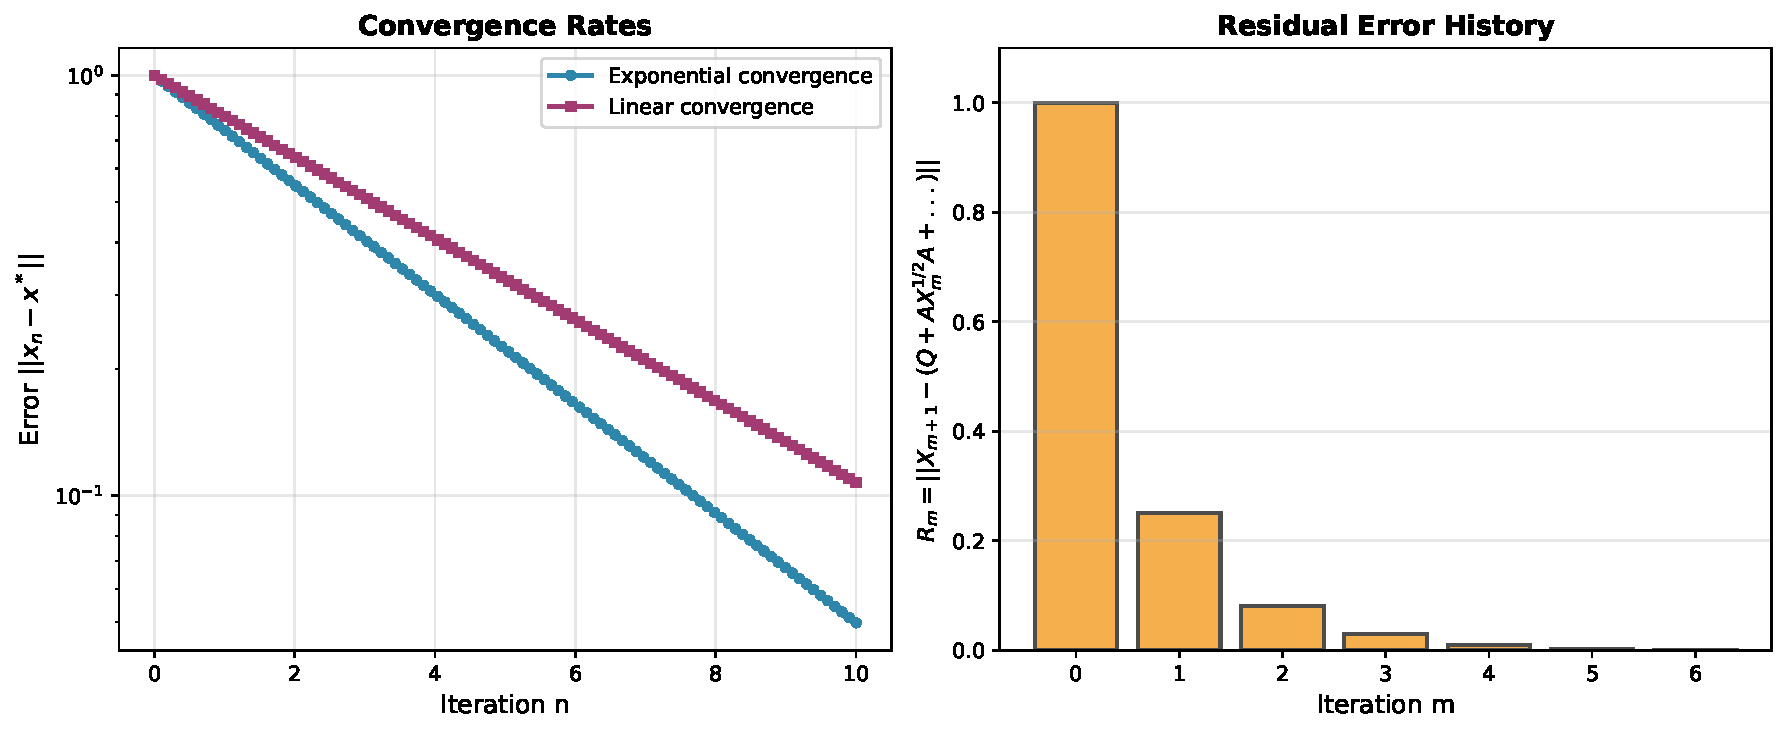
\includegraphics[width=0.95\textwidth]{fig_01_iterative_convergence.pdf}
  \end{center}

  \vspace{0.2cm}
  \small
  The left panel shows exponential vs. linear convergence rates.
  The right panel displays residual error history over iterations.
\end{frame}

%===============================================================================
\section{Iterative Methods for Finding Fixed Points}
%===============================================================================

\begin{frame}{Mann Iteration}
  \begin{definition}[Mann Iteration (1953)]
    For a mapping $T: D \to D$, the Mann iteration is defined by:
    \[
      x_{n+1} = (1 - \alpha_n) x_n + \alpha_n T(x_n),
      \quad n = 0, 1, 2, \ldots
    \]
    where $\{\alpha_n\}$ is a sequence of parameters with $0 \leq \alpha_n \leq 1$.
  \end{definition}

  \vspace{0.3cm}

  \begin{block}{Properties}
    \item When $\alpha_n = 1$: recovers Picard iteration.
    \item When $0 < \alpha_n < 1$: provides convex combination (damping).
    \item Choice of $\{\alpha_n\}$ affects convergence:
      \begin{itemize}
        \item Constant $\alpha_n = \alpha$: easier analysis
        \item Variable $\{\alpha_n\}$: may accelerate convergence
      \end{itemize}
  \end{block}

  \vspace{0.3cm}

  \begin{theorem}[Convergence of Mann Iteration]
    Under appropriate conditions on $T$ and $\{\alpha_n\}$, the Mann iteration
    converges to a fixed point of $T$.
  \end{theorem}
\end{frame}

\begin{frame}[fragile]{Mann Iteration Example}
  \begin{block}{Python Implementation}
    \begin{lstlisting}
import numpy as np

def mann_iteration(T, x0, alpha=0.5, max_iter=100, tol=1e-8):
    """Mann iteration for fixed point approximation"""
    x = x0
    history = [x]

    for n in range(max_iter):
        T_x = T(x)
        x_new = (1 - alpha) * x + alpha * T_x

        if np.linalg.norm(x_new - x) < tol:
            print(f"Converged in {n+1} iterations")
            break

        x = x_new
        history.append(x)

    return x, np.array(history)

# Example: T(x) = 0.5*x + 0.3*sin(x)
T = lambda x: 0.5*x + 0.3*np.sin(x)
x_fixed, history = mann_iteration(T, x0=0.0)
    \end{lstlisting}
  \end{block}
\end{frame}

\begin{frame}{Ishikawa Iteration}
  \begin{definition}[Ishikawa Iteration (1974)]
    The Ishikawa iteration is a two-step scheme:
    \begin{align}
      y_n &= (1 - \beta_n) x_n + \beta_n T(x_n), \\
      x_{n+1} &= (1 - \alpha_n) x_n + \alpha_n T(y_n),
    \end{align}
    where $\{\alpha_n\}$ and $\{\beta_n\}$ are parameter sequences.
  \end{definition}

  \vspace{0.3cm}

  \begin{block}{Properties}
    \item Generalizes Mann iteration (recovers it when $\beta_n = 0$).
    \item Potential for faster convergence with two parameters.
    \item More computational cost (two applications of $T$ per iteration).
  \end{block}

  \vspace{0.3cm}

  \begin{block}{Comparison of Methods}
    \begin{tabular}{lll}
      \hline
      Method & Iterations & Evaluations of $T$ \\
      \hline
      Picard & $x_{n+1} = T(x_n)$ & 1 per iteration \\
      Mann & $x_{n+1} = (1-\alpha)x_n + \alpha T(x_n)$ & 1 per iteration \\
      Ishikawa & Two-step scheme & 2 per iteration \\
      \hline
    \end{tabular}
  \end{block}
\end{frame}

\begin{frame}{Noor Iteration}
  \begin{definition}[Noor Iteration (1997)]
    A three-step iteration scheme:
    \begin{align}
      y_n &= (1 - \beta_n) x_n + \beta_n T(x_n), \\
      z_n &= (1 - \gamma_n) y_n + \gamma_n T(y_n), \\
      x_{n+1} &= (1 - \alpha_n) z_n + \alpha_n T(z_n),
    \end{align}
  \end{definition}

  \vspace{0.3cm}

  \begin{block}{Properties}
    \item Potentially faster convergence with three parameters.
    \item Increased computational cost (3 evaluations of $T$ per iteration).
    \item Useful for certain nonlinear operators and nonexpansive mappings.
  \end{block}
\end{frame}

%===============================================================================
\section{Applications to Differential Equations}
%===============================================================================

\begin{frame}[allowframebreaks]{Two-Point Boundary Value Problems}
  \begin{problem}
    Consider the boundary value problem:
    \begin{align}
      x''(t) &= f(t, x(t), x'(t)), \quad 0 \leq t \leq T, \\
      x(0) &= \alpha, \quad x(T) = \beta.
    \end{align}
  \end{problem}

  \vspace{0.3cm}

  \begin{solution}
    Transform to an integral equation:
    \[
      x(t) = \alpha + \frac{(\beta - \alpha)t}{T} - \int_0^T G(t,s) f(s, x(s), x'(s)) \, ds,
    \]
    where $G(t,s)$ is the Green's function:
    \[
      G(t,s) = \begin{cases}
        \frac{s(T-t)}{T} & 0 \leq s \leq t \leq T \\
        \frac{t(T-s)}{T} & 0 \leq t \leq s \leq T
      \end{cases}
    \]
  \end{solution}

  \framebreak

  \begin{block}{Fixed Point Formulation}
    Define the operator $F: C^1[0,T] \to C^1[0,T]$ by:
    \[
      (Fx)(t) = \alpha + \frac{(\beta - \alpha)t}{T} - \int_0^T G(t,s) f(s, x(s), x'(s)) \, ds.
    \]

    The boundary value problem solution is a fixed point of $F$:
    \[
      F(x) = x \quad \iff \quad x \text{ solves the BVP}.
    \]
  \end{block}

  \vspace{0.3cm}

  \begin{theorem}
    Under appropriate boundedness and continuity conditions on $f$ and the
    Green's function, $F$ is continuous and compact. By Schauder's fixed
    point theorem, $F$ has at least one fixed point.
  \end{theorem}
\end{frame}

\begin{frame}{Periodic Solution Problem}
  \begin{problem}
    Find periodic solutions to:
    \begin{equation}
      \frac{dx}{dt} = f(t, x(t)), \quad x(0) = x(p),
    \end{equation}
    where $p > 0$ is the period and $f(t, x)$ is periodic in $t$ with period $p$.
  \end{problem}

  \vspace{0.4cm}

  \begin{solution}
    Define the operator $F: C[0,p] \to C[0,p]$ by:
    \[
      (Fx)(t) = x_0 + \int_0^t f(s, x(s)) \, ds,
    \]
    where the periodicity condition imposes additional constraints.

    The Poincaré operator (period map) can be analyzed to show existence
    of periodic solutions via fixed point theory.
  \end{solution}
\end{frame}

%===============================================================================
\section{Applications to Integral Equations}
%===============================================================================

\begin{frame}{Hammerstein Integral Equations}
  \begin{definition}[Hammerstein Equation]
    An equation of the form:
    \[
      x(t) = \lambda \int_a^b K(t,s) f(s, x(s)) \, ds + g(t),
    \]
    where:
    \begin{itemize}
      \item $K(t,s)$ is the kernel (typically continuous)
      \item $f(s, x)$ is a nonlinearity
      \item $\lambda$ is a parameter
      \item $g(t)$ is a given function
    \end{itemize}
  \end{definition}

  \vspace{0.4cm}

  \begin{block}{Fixed Point Formulation}
    The Hammerstein equation can be written as a fixed point problem:
    \[
      x = T(x),
    \]
    where $(T x)(t) = \lambda \int_a^b K(t,s) f(s, x(s)) \, ds + g(t)$.
  \end{block}
\end{frame}

\begin{frame}[fragile]{Hammerstein Equation: Numerical Example}
  \begin{block}{Example Setup}
    Consider:
    \[
      x(t) = \lambda \int_0^1 (t + s) \exp(-x(s)) \, ds + t
    \]
  \end{block}

  \vspace{0.3cm}

  \begin{block}{Python Solution}
    \begin{lstlisting}
from scipy.integrate import quad

def hammerstein_operator(x_func, lam=0.5):
    """Hammerstein operator application"""
    def T(t):
        integrand = lambda s: (t + s) * np.exp(-x_func(s))
        result, _ = quad(integrand, 0, 1)
        return lam * result + t
    return T

# Fixed point iteration
def solve_hammerstein(lam, max_iter=50):
    # Start with x_0(t) = t
    x = lambda t: t

    for n in range(max_iter):
        x_new = hammerstein_operator(x, lam)
        # Check convergence
        # ...

    return x
    \end{lstlisting}
  \end{block}
\end{frame}

\begin{frame}{Urysohn Integral Equations}
  \begin{definition}[Urysohn Equation]
    An equation of the form:
    \[
      x(t) = \int_\Omega f(t, s, x(s)) \, ds,
    \]
    where $f: \Omega \times \Omega \times \mathbb{R} \to \mathbb{R}$ is a given kernel.
  \end{definition}

  \vspace{0.4cm}

  \begin{remark}
    The Hammerstein equation is a special case where $f(t,s,x) = K(t,s) g(x)$.
  \end{remark}

  \vspace{0.4cm}

  \begin{theorem}[Existence of Solutions]
    If:
    \begin{enumerate}
      \item $f$ is continuous on $\Omega \times \Omega \times \mathbb{R}$,
      \item $f$ satisfies a Lipschitz condition in the third variable,
      \item $\int_\Omega |f(t,s,0)| \, ds \leq M$ for some constant $M$,
    \end{enumerate}
    then the Urysohn equation has at least one solution in $C(\Omega)$.
  \end{theorem}
\end{frame}

%===============================================================================
\section{Numerical Examples and Convergence Rates}
%===============================================================================

\begin{frame}{Sequence Convergence Behaviors}
  \begin{center}
    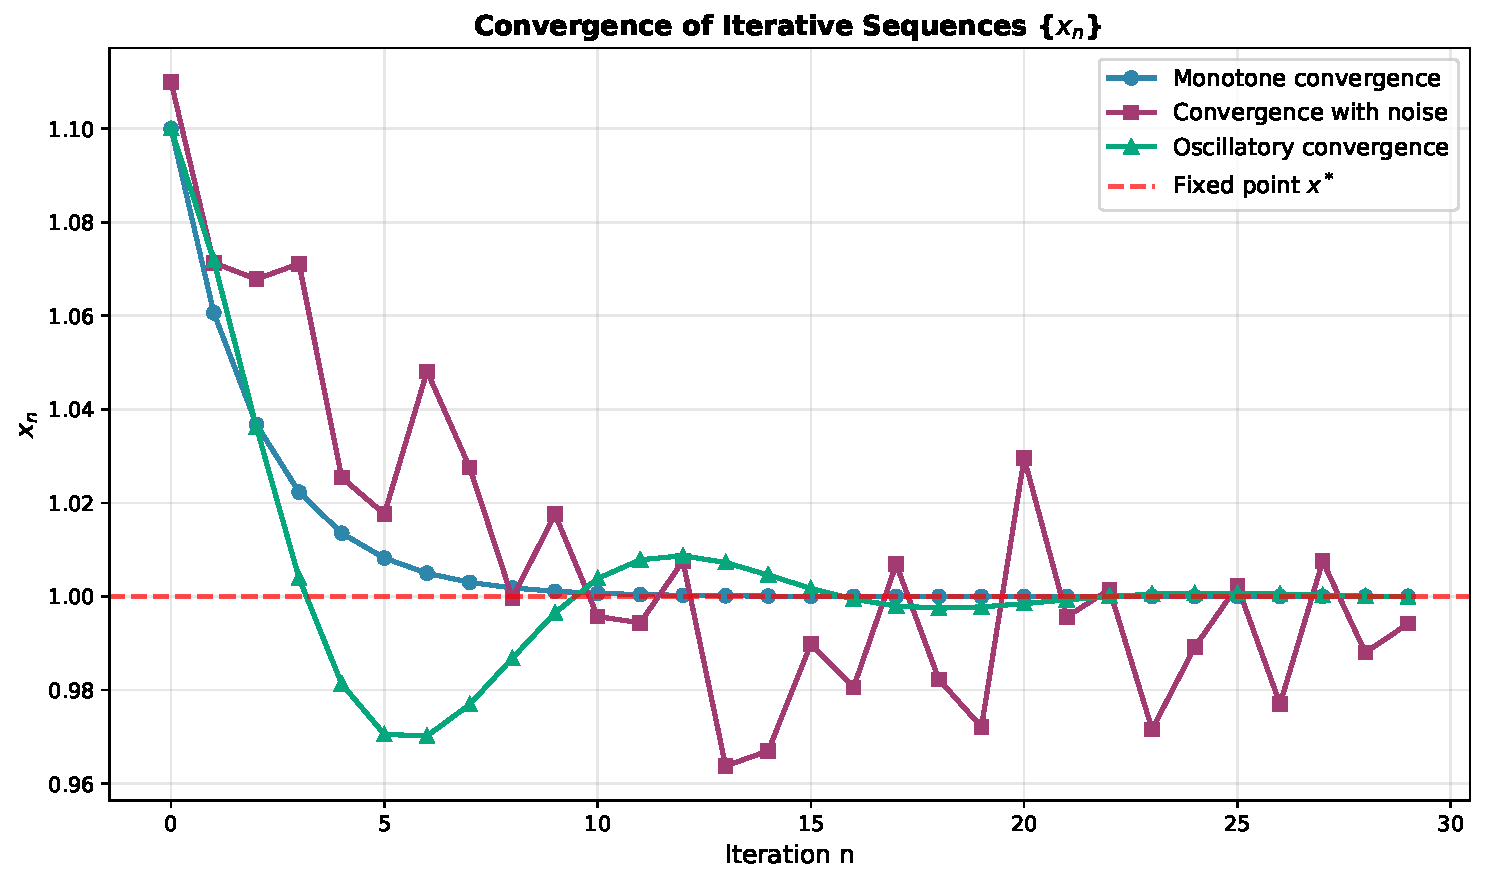
\includegraphics[width=0.95\textwidth]{fig_04_sequence_convergence.pdf}
  \end{center}

  \vspace{0.2cm}
  \small
  Different iterative sequences exhibit different convergence patterns:
  monotone convergence, convergence with noise, and oscillatory convergence.
\end{frame}

\begin{frame}{Fixed Point Iteration Visualization}
  \begin{center}
    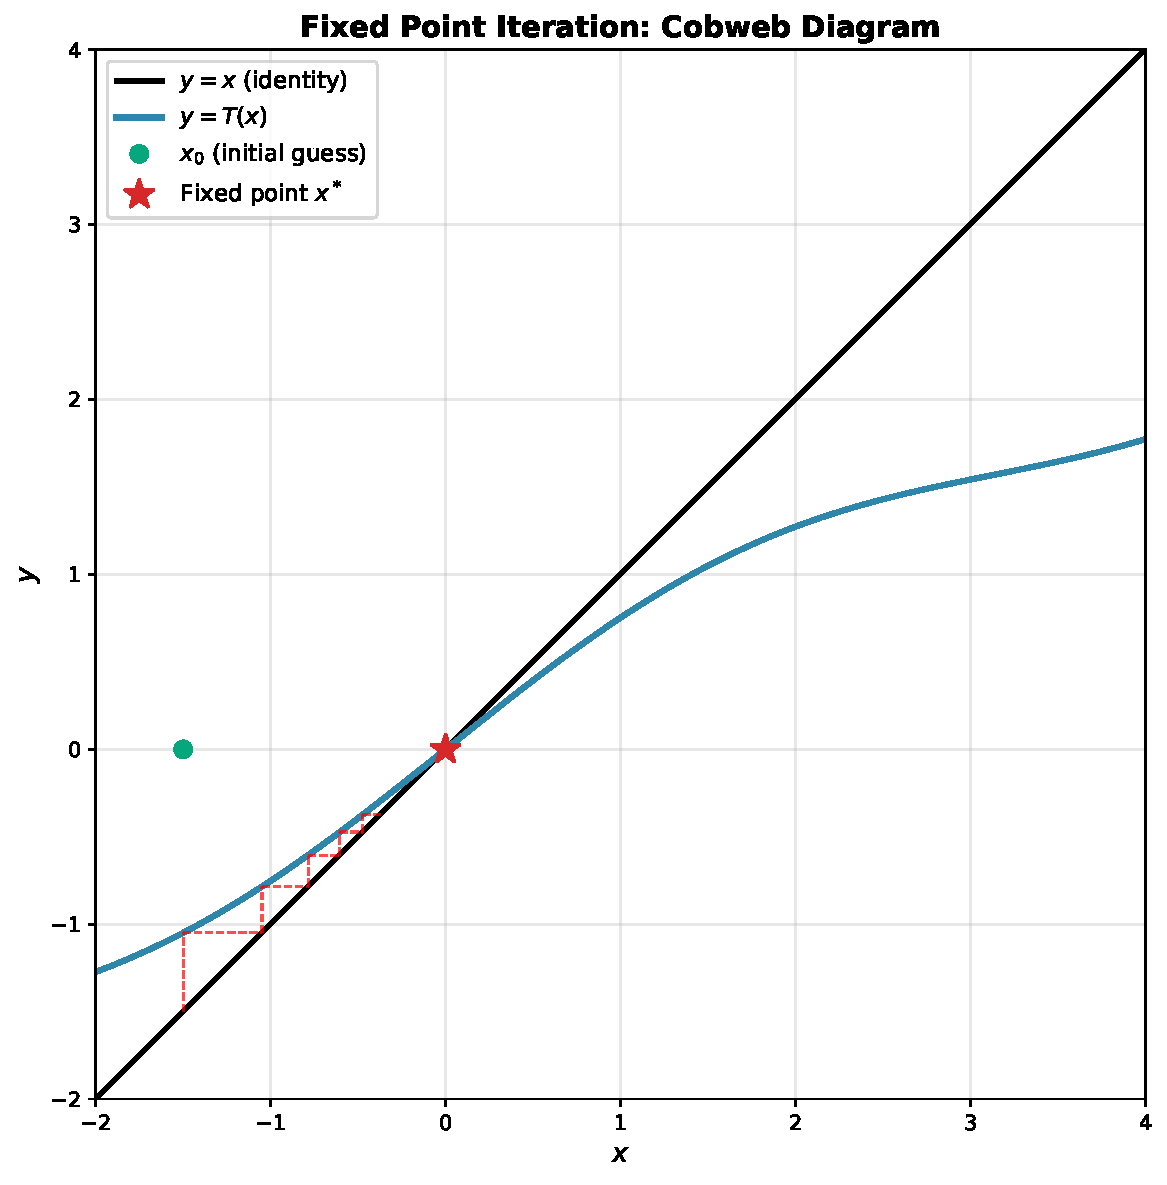
\includegraphics[width=0.85\textwidth]{fig_02_fixed_point_iteration.pdf}
  \end{center}

  \vspace{0.2cm}
  \small
  The cobweb diagram illustrates how iterates approach the fixed point
  at the intersection of $y = x$ and $y = T(x)$.
\end{frame}

\begin{frame}[fragile]{Computational Example: Matrix Fixed Point}
  \begin{block}{Problem}
    Solve $X = Q + AX^{1/2}A^* + BX^{-1}B^*$ using Picard iteration.
  \end{block}

  \begin{lstlisting}
import numpy as np
from scipy.linalg import sqrtm

def matrix_fixed_point(Q, A, B, X0, max_iter=100, tol=1e-8):
    """Solve matrix fixed point equation iteratively"""
    X = X0.copy()

    for m in range(max_iter):
        X_sqrt = sqrtm(X)
        X_inv = np.linalg.inv(X)

        # Picard step: X_{m+1} = T(X_m)
        X_new = Q + A @ X_sqrt @ A.T + B @ X_inv @ B.T

        # Compute residual
        residual = np.linalg.norm(X_new - X)

        if residual < tol:
            print(f"Converged in {m+1} iterations")
            return X_new

        X = X_new

    return X
  \end{lstlisting}
\end{frame}

%===============================================================================
\section{Advanced Topics}
%===============================================================================

\begin{frame}{Nonexpansive Mappings}
  \begin{definition}[Nonexpansive Mapping]
    A mapping $T: D \to X$ is \textbf{nonexpansive} if:
    \[
      \|T(x) - T(y)\| \leq \|x - y\|
      \quad \text{for all } x, y \in D.
    \]
  \end{definition}

  \vspace{0.4cm}

  \begin{remark}
    \textbf{Key difference from contractions:}
    \begin{itemize}
      \item Nonexpansive: contraction rate $\lambda = 1$ (not strictly less than 1).
      \item Banach theorem does not directly apply!
      \item Requires additional structure (e.g., compactness, normal structure).
    \end{itemize}
  \end{remark}

  \vspace{0.4cm}

  \begin{theorem}[Schauder Fixed Point Theorem]
    If $T: K \to K$ is continuous and $K$ is a nonempty compact convex subset
    of a Banach space, then $T$ has a fixed point in $K$.
  \end{theorem}
\end{frame}

\begin{frame}{Quasi-Nonexpansive Mappings}
  \begin{definition}[Quasi-Nonexpansive]
    A mapping $T$ is quasi-nonexpansive if it has a fixed point $x^*$ and:
    \[
      \|T(x) - x^*\| \leq \|x - x^*\|
      \quad \text{for all } x \in D.
    \]
  \end{definition}

  \vspace{0.4cm}

  \begin{block}{Properties}
    \item Weaker than nonexpansive (doesn't require $\|T(x)-T(y)\| \leq \|x-y\|$ for all $x,y$).
    \item Guarantees monotone convergence to the fixed point.
    \item Examples: projections onto closed convex sets.
  \end{block}

  \vspace{0.4cm}

  \begin{theorem}
    If $T$ is quasi-nonexpansive and Mann iteration is used with appropriate
    parameters $\{\alpha_n\}$, then $\{x_n\}$ converges to the fixed point.
  \end{theorem}
\end{frame}

\begin{frame}{Hybrid Methods and Operator Splitting}
  \begin{block}{Motivation}
    For complex operators $T = T_1 + T_2$ or $T = T_1 \circ T_2$,
    apply iterations to individual components.
  \end{block}

  \vspace{0.3cm}

  \begin{definition}[Operator Splitting]
    Instead of:
    \[
      x_{n+1} = T(x_n),
    \]
    use:
    \begin{align}
      x_{n+1} &= T_1(T_2(x_n)), \quad \text{(Alternating)} \\
      x_{n+1} &= \lambda T_1(x_n) + (1-\lambda) T_2(x_n), \quad \text{(Convex combination)}
    \end{align}
  \end{definition}

  \vspace{0.3cm}

  \begin{block}{Applications}
    Useful for:
    \begin{itemize}
      \item Proximal operator splitting in optimization.
      \item Douglas-Rachford algorithm for sum of operators.
      \item Alternating projections for feasibility problems.
    \end{itemize}
  \end{block}
\end{frame}

%===============================================================================
\section{Summary and Applications}
%===============================================================================

\begin{frame}{Summary of Key Results}
  \begin{enumerate}
    \item \textbf{Banach Contraction Principle}: $\lambda$-contractions have unique
          fixed points reachable by Picard iteration with exponential convergence.

    \vspace{0.25cm}

    \item \textbf{Iterative Methods}: Mann, Ishikawa, and Noor iterations generalize
          Picard iteration with damping parameters for improved convergence.

    \vspace{0.25cm}

    \item \textbf{Differential Equations}: Boundary value and periodic solution problems
          reduce to fixed point equations via Green's functions.

    \vspace{0.25cm}

    \item \textbf{Integral Equations}: Hammerstein and Urysohn equations are fixed
          point problems in function spaces.

    \vspace{0.25cm}

    \item \textbf{Nonexpansive and Quasi-Nonexpansive}: Extended theory for mappings
          not satisfying strict contractiveness.
  \end{enumerate}
\end{frame}

\begin{frame}{Applications Across Disciplines}
  \begin{block}{Numerical Analysis}
    \begin{itemize}
      \item Solving nonlinear equations (Newton's method, fixed point iteration)
      \item Eigenvalue problems and spectral computations
      \item Matrix equations and tensor computations
    \end{itemize}
  \end{block}

  \begin{block}{Optimization}
    \begin{itemize}
      \item Proximal methods and forward-backward splitting
      \item Alternating direction method of multipliers (ADMM)
      \item Stochastic gradient descent and online learning
    \end{itemize}
  \end{block}

  \begin{block}{Engineering and Physics}
    \begin{itemize}
      \item Control system design and feedback loops
      \item Chemical reactor models
      \item Fluid dynamics and partial differential equations
    \end{itemize}
  \end{block}
\end{frame}

\begin{frame}{Open Problems and Future Directions}
  \begin{enumerate}
    \item \textbf{Acceleration Techniques}: How to enhance convergence rates
          using preprocessing, extrapolation, or Krylov subspace methods?

    \vspace{0.3cm}

    \item \textbf{Nonlinear Operators}: Theory for more general nonlinear structures
          beyond contractions and nonexpansive mappings.

    \vspace{0.3cm}

    \item \textbf{Stochastic Algorithms}: Convergence analysis for randomized
          and stochastic fixed point iterations.

    \vspace{0.3cm}

    \item \textbf{Distributed Computing}: Fixed point methods for parallel and
          distributed computing in large-scale problems.

    \vspace{0.3cm}

    \item \textbf{Machine Learning}: Applications to deep learning training
          algorithms and neural network optimization.
  \end{enumerate}
\end{frame}

\begin{frame}[allowframebreaks]{References}
  \small
  \begin{thebibliography}{99}
    \bibitem{Pathak2018}
    Pathak, H. K. (2018). An Introduction to Nonlinear Analysis and Fixed Point Theory.
    Springer-Verlag.

    \bibitem{Banach1922}
    Banach, S. (1922). Sur les opérations dans les ensembles abstraits et leur application aux équations intégrales.
    Fundamenta Mathematicae, 3(1), 133-181.

    \bibitem{Mann1953}
    Mann, W. A. (1953). Mean value methods in iteration.
    Proceedings of the American Mathematical Society, 4(3), 506-510.

    \bibitem{Ishikawa1974}
    Ishikawa, S. (1974). Fixed points by a new iteration method.
    Proceedings of the American Mathematical Society, 44(1), 147-150.

    \bibitem{Noor1997}
    Noor, M. A. (1997). New approximation schemes for general variational inequalities.
    Journal of Mathematical Analysis and Applications, 251(1), 217-229.

    \bibitem{Berinde2007}
    Berinde, V. (2007). Iterative Approximation of Fixed Points.
    Springer-Verlag.
  \end{thebibliography}
\end{frame}

\end{document}
